% Created 2020-10-05 Mon 16:17
% Intended LaTeX compiler: pdflatex
\documentclass[10pt,t]{beamer}
\usepackage[utf8]{inputenc}
\usepackage[T1]{fontenc}
\usepackage{graphicx}
\usepackage{grffile}
\usepackage{longtable}
\usepackage{wrapfig}
\usepackage{rotating}
\usepackage{amsmath}
\usepackage{textcomp}
\usepackage{amssymb}
\usepackage{capt-of}
\usepackage{hyperref}
\usetheme{default}
\author{L. Larrabee Strow}
\date{\today}
\title{\large AIRS RTA and BT Tuning:}
\subtitle{\footnotesize{RTA Tuning Telecon}}
\date{\vspace{0.1in}\footnotesize{June 25, 2020 \vfill}}
\author{L. Larrabee Strow}
\input beamer_setup
\usetheme{metropolis}
\metroset{titleformat title=allcaps}
\setbeamercolor{alert}{fg=maroon}
\renewcommand{\UrlFont}{\small\tt}
\renewcommand*{\UrlFont}{\footnotesize}
\tolerance=1000
\RequirePackage{fancyvrb}
\DefineVerbatimEnvironment{verbatim}{Verbatim}{fontsize=\footnotesize}
\begin{document}

\maketitle
\addtobeamertemplate{block begin}{
  \setlength{\parsep}{0pt}
  \setlength{\topsep}{3pt plus 2pt minus 2.5pt}
  \setlength{\itemsep}{0pt plus 0pt minus 2pt}
  \setlength{\partopsep}{2pt}
}

\begin{frame}[label={sec:org472f9d3}]{Introduction}
\begin{itemize}
\item 17 days of AIRS clear ocean scene radiances are compared to ECMWF simulations
\item Three RTA variants tested:
\begin{itemize}
\item L1c RTA
\item L1b RTA as tuned for V6 Level 2 retrievals
\item L1b RTA without tuning
\end{itemize}
\item The L1c RTA uses HITRAN 2016 and new (improvements?) to the continuum and line mixing
\item The L1b RTA is circa 2008
\item Conclusions here assume ECMWF is "truth".  Better than 5\% --> 0.3K?
\end{itemize}
\end{frame}
\begin{frame}[label={sec:orgf207f3e}]{Longwave Biases: All RTAs}
\begin{center}
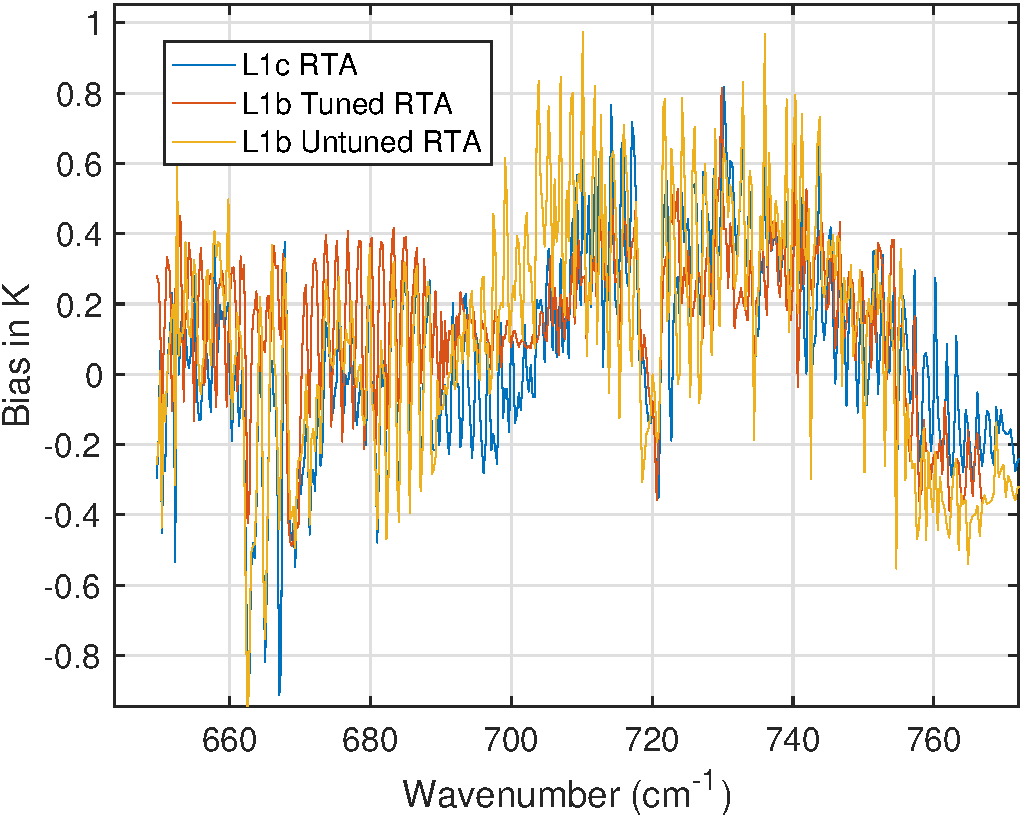
\includegraphics[width=0.75\linewidth]{./bias_3rta_lw.pdf}
\end{center}
\end{frame}
\begin{frame}[label={sec:org87db84f}]{Longwave Biases w/o L1btuning RTA}
L1c RTA appears a bit better.  (Note fill channels included!)
\begin{center}
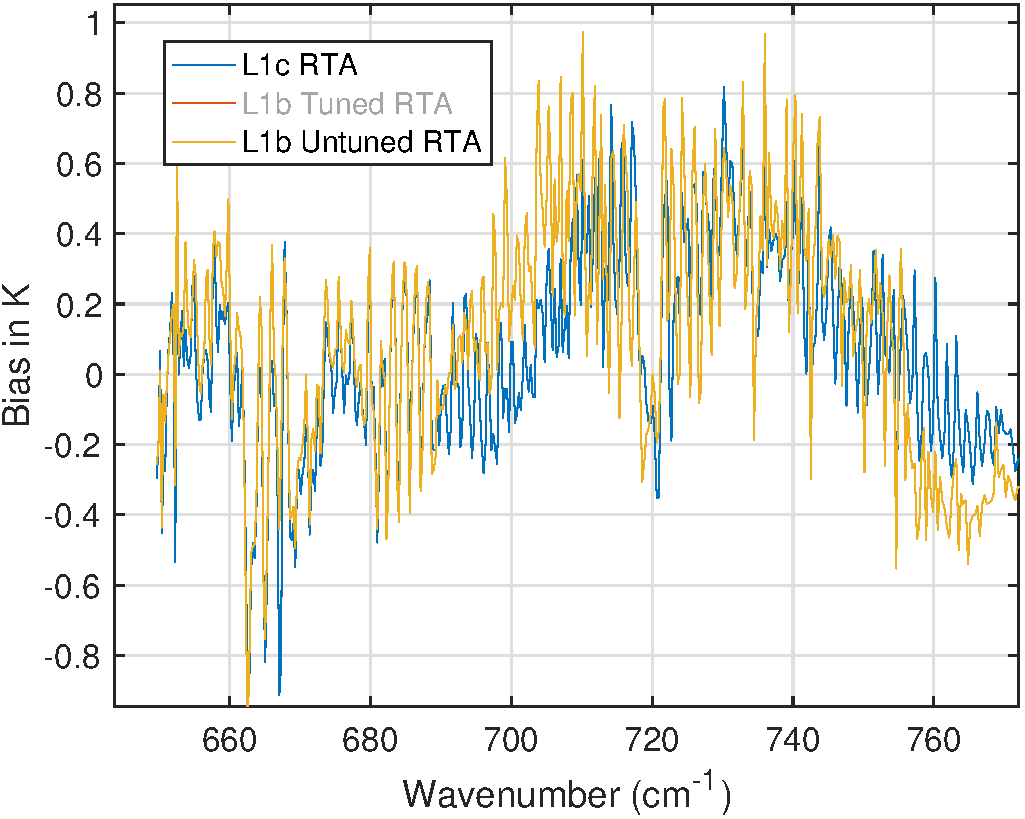
\includegraphics[width=0.75\linewidth]{./bias_3rta_lw_noL1btuning.pdf}
\end{center}
\end{frame}
\begin{frame}[label={sec:org2af980b}]{Longwave Biases just L1btuning RTA}
Tuning removes biases mostly to levels lower than either RTA, esp. for trop. channels
\begin{center}
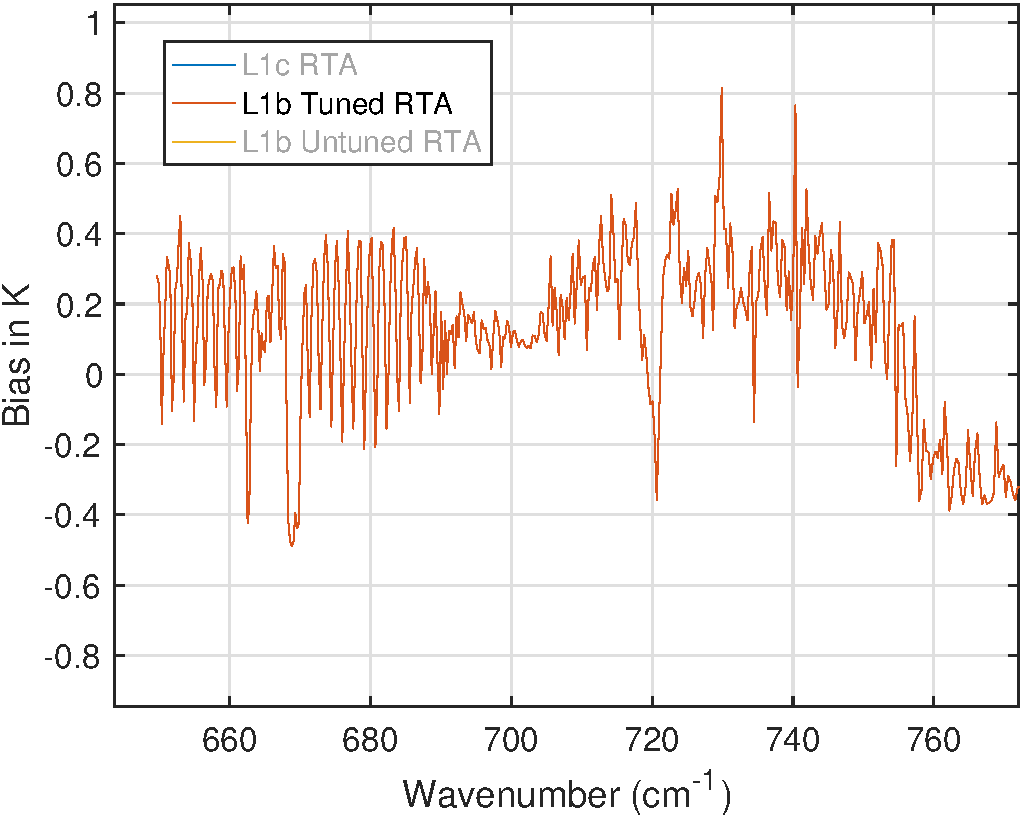
\includegraphics[width=0.75\linewidth]{./bias_3rta_lw_justL1btuning.pdf}
\end{center}
\end{frame}
\begin{frame}[label={sec:org68cebb3}]{Midwave Biases: All RTAs}
L1c slightly "worse" than L1b.  Tuned L1b high bias, but smooth with \wn
\begin{center}
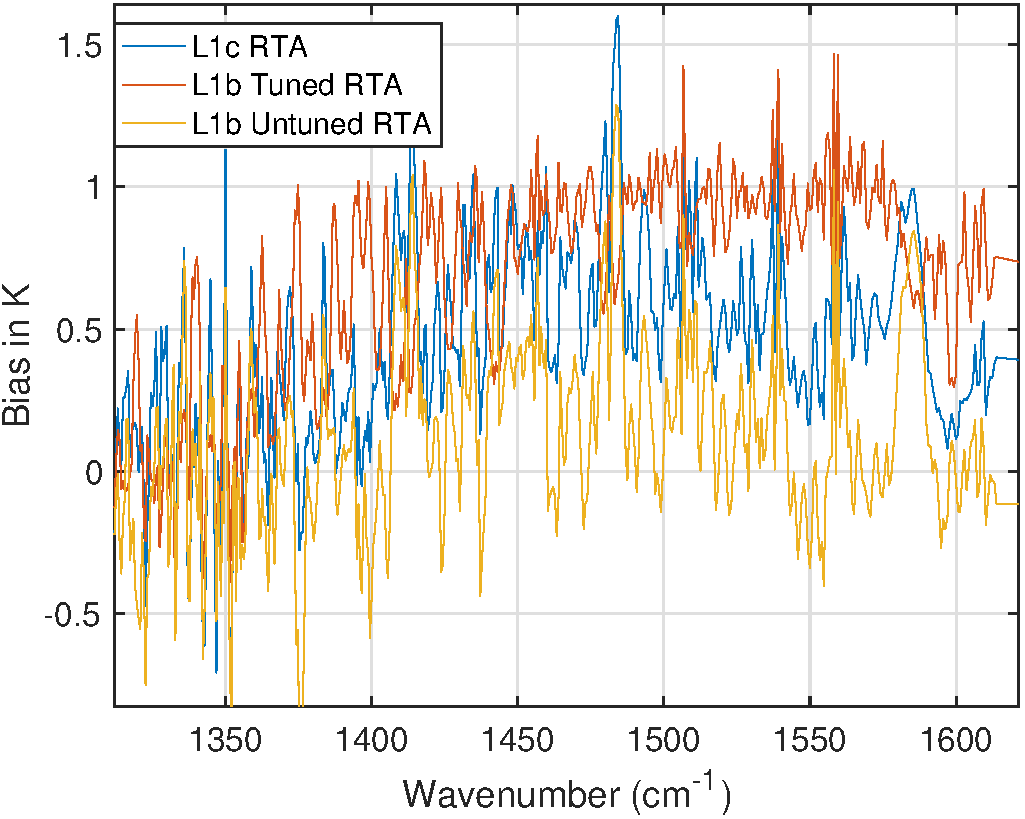
\includegraphics[width=0.75\linewidth]{./bias_3rta_mw.pdf}
\end{center}
\end{frame}
\begin{frame}[label={sec:org5d2824b}]{Midwave Biases w/o L1btuning RTA}
Mixed bag: although L1b untuned biases are smaller on average
\begin{center}
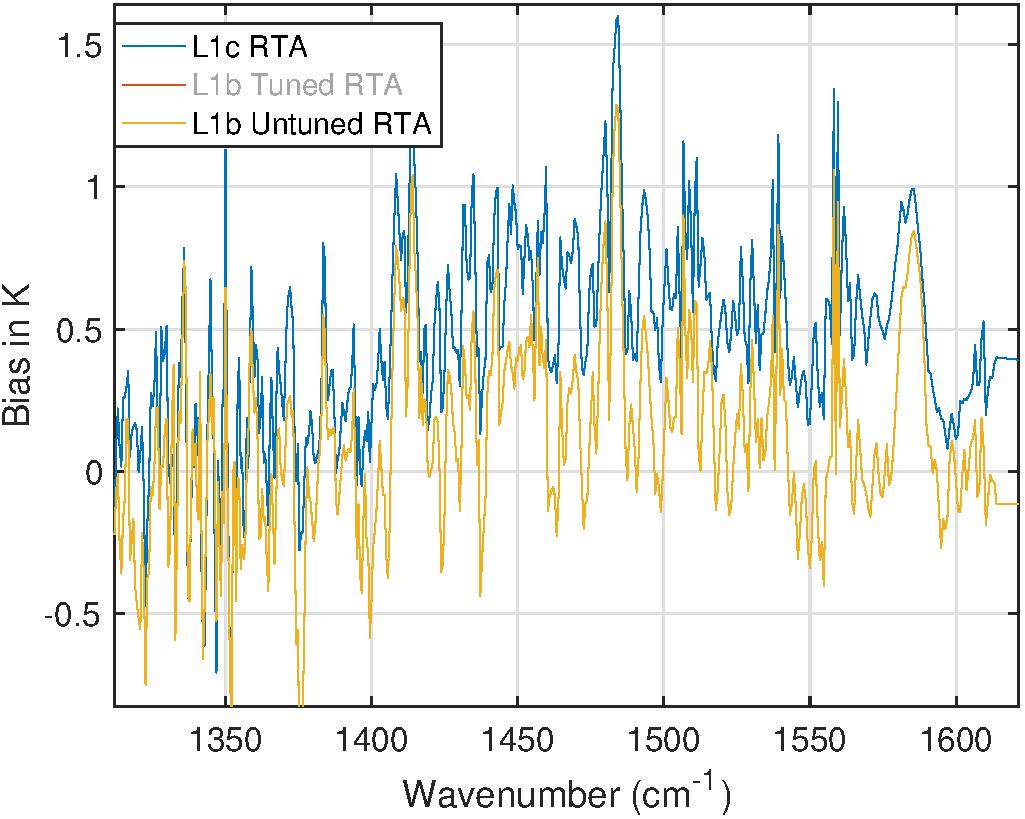
\includegraphics[width=0.75\linewidth]{./bias_3rta_mw_noL1btuning.pdf}
\end{center}
\end{frame}
\begin{frame}[label={sec:org22ce356}]{Midwave Biases Just L1btuning RTA}
Clear that L1b tuning removes channel-to-channel variability (help convergence?)
\begin{center}
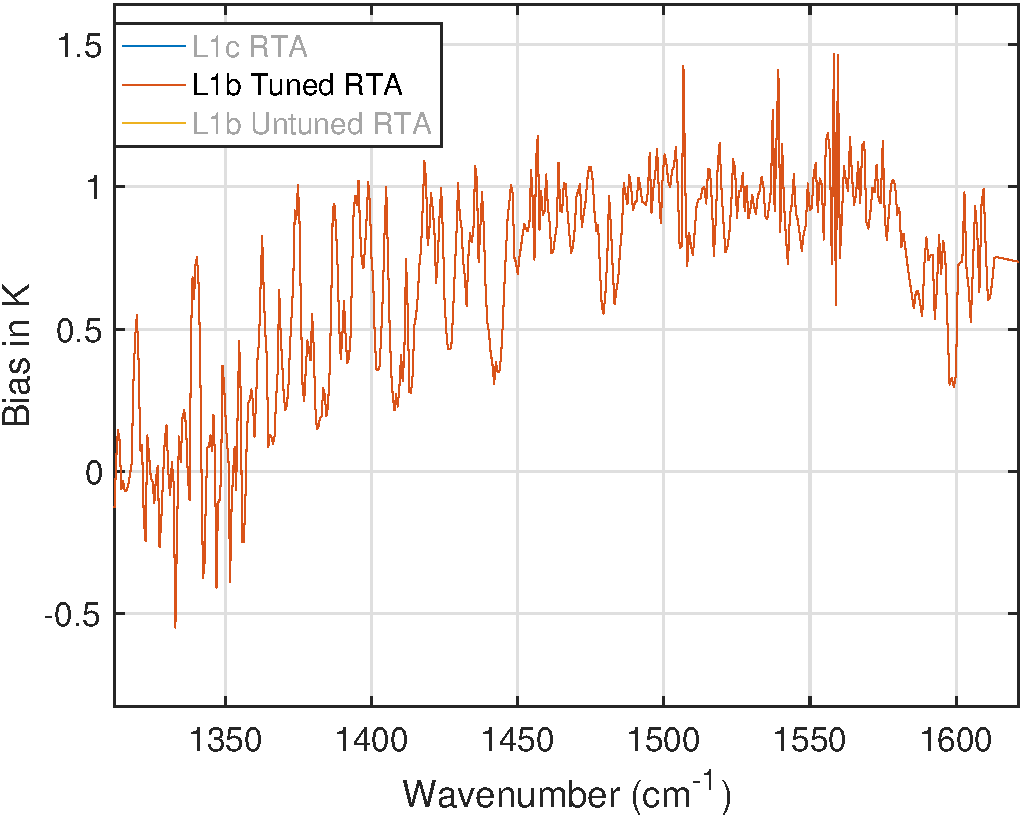
\includegraphics[width=0.75\linewidth]{./bias_3rta_mw_justL1btuning.pdf}
\end{center}
\end{frame}
\begin{frame}[label={sec:org047c8ba}]{650-700 \wn Biases vs BTobs}
Strat channels: L1b tuned clear bias trend with BTobs, unlike untuned RTAs
\begin{center}
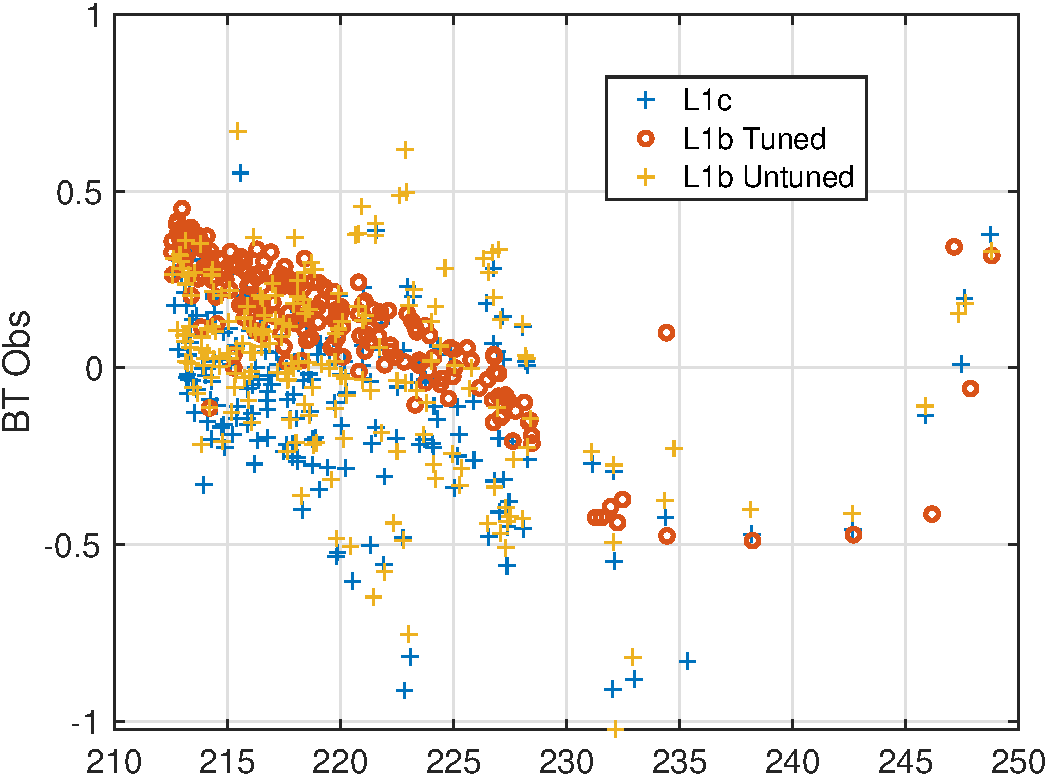
\includegraphics[width=0.75\linewidth]{./bias_vs_btobs_650-700.pdf}
\end{center}
\end{frame}
\begin{frame}[label={sec:org6447e1f}]{1320-1614 \wn Biases vs BTobs}
Similarly for water band, L1b tuned clear bias dependence on BTobs
\begin{center}
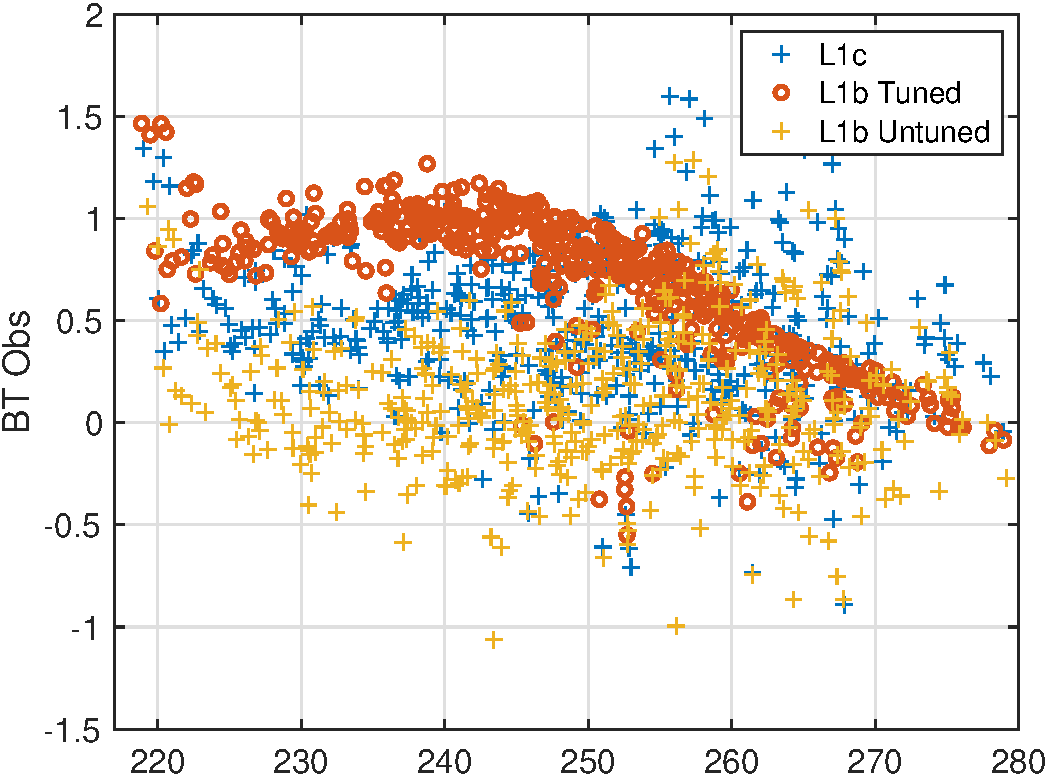
\includegraphics[width=0.75\linewidth]{./bias_vs_btobs_1320-1614.pdf}
\end{center}
\end{frame}
\begin{frame}[label={sec:org9697316}]{Longwave Bias Standard Deviations (with Latitude)}
L1c stds often smaller than L1b (tuned or untuned)
\begin{center}
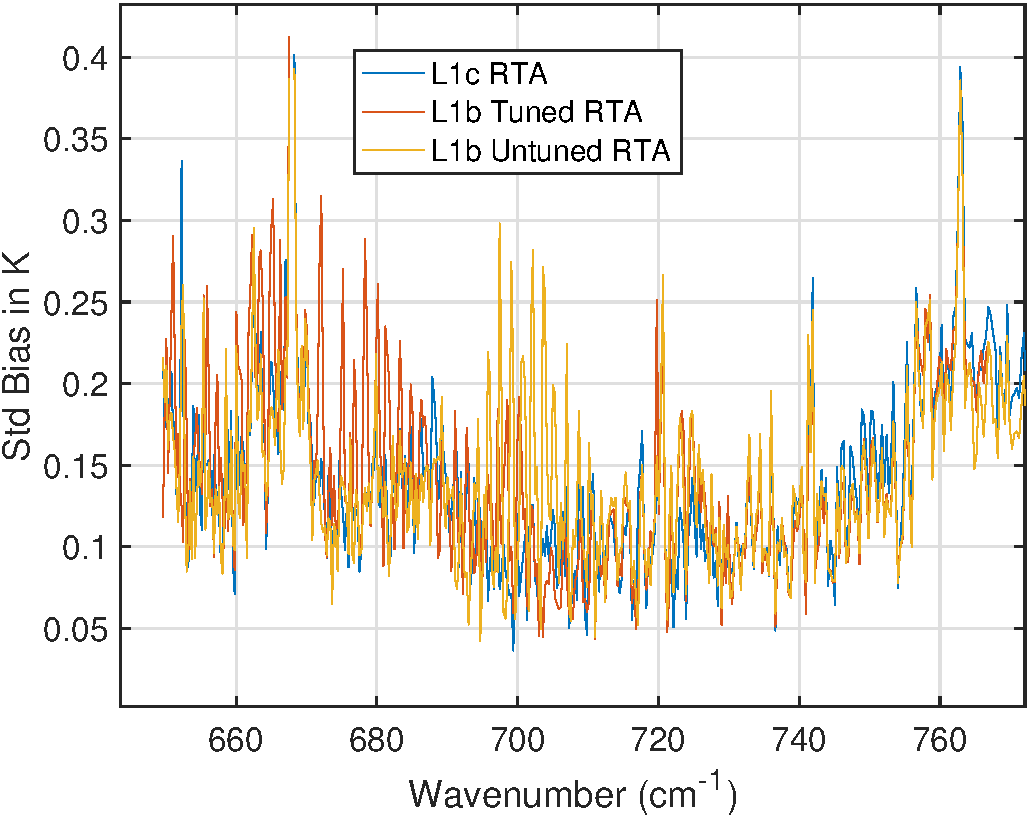
\includegraphics[width=0.75\linewidth]{./std_3rta_lw.pdf}
\end{center}
\end{frame}
\begin{frame}[label={sec:org0f46d77}]{Longwave Bias Stds w/o L1btuning RTA}
Tropopause region much smaller STD for L1c vs L1b (untuned)
\begin{center}
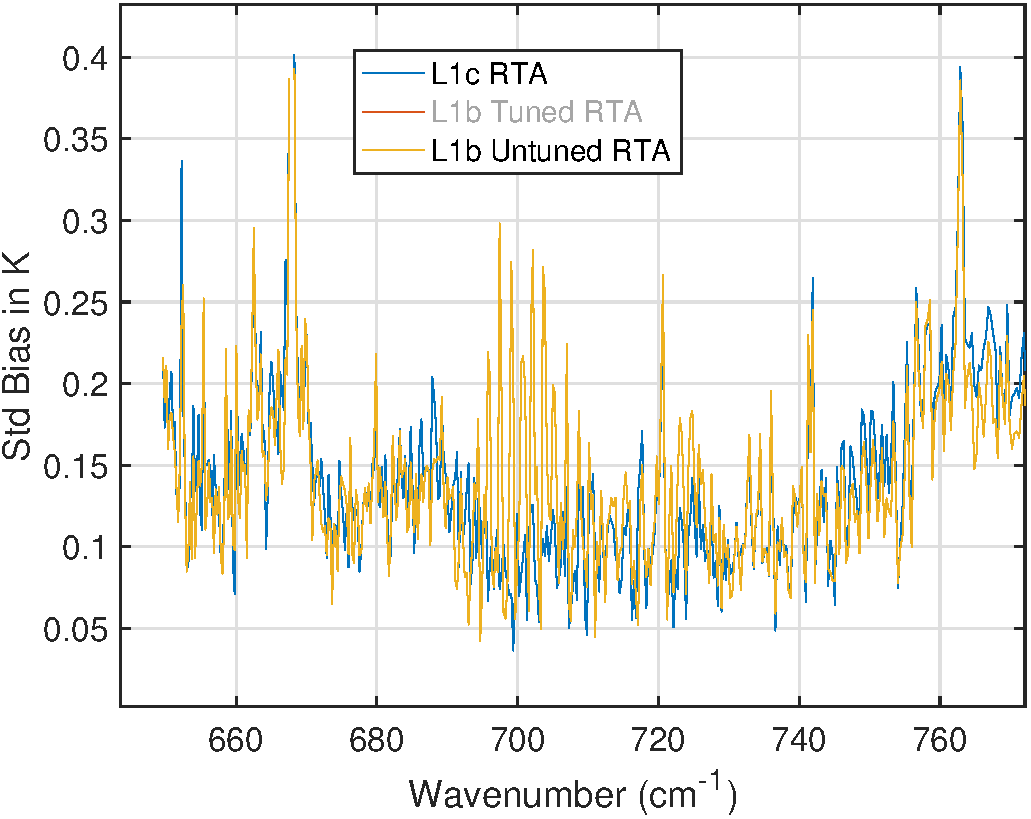
\includegraphics[width=0.75\linewidth]{./std_3rta_lw_noL1btuning.pdf}
\end{center}
\end{frame}
\begin{frame}[label={sec:orga29dad3}]{Longwave Bias Stds w/o L1b(untuned) RTA}
L1b tuning mostly removes higher L1b STD, but strat channels worse
\begin{center}
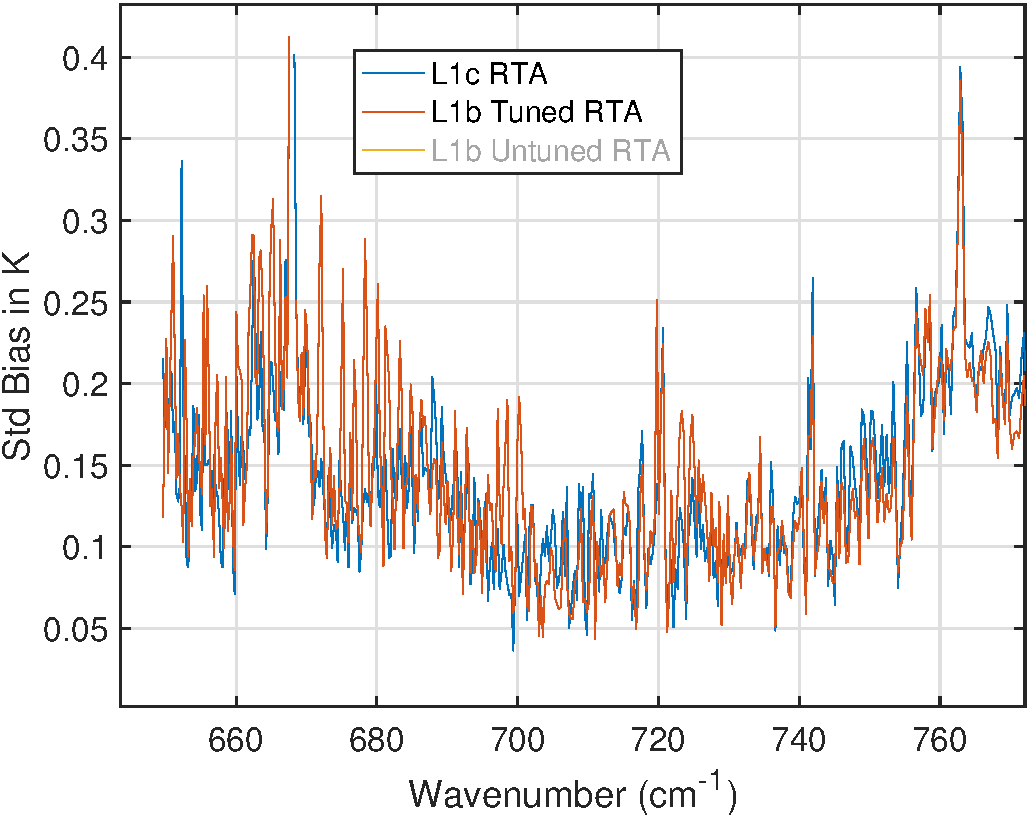
\includegraphics[width=0.75\linewidth]{./std_3rta_lw_nol1b_untuned.pdf}
\end{center}
\end{frame}
\begin{frame}[label={sec:orgfcad398}]{Midwave Bias Stds: All RTAs}
\begin{itemize}
\item Very clear: L1c RTA channel-to-channel STDs very similar
\item L1b tuned STDs far higher than L1c, L1b untuned even lower
\end{itemize}
\begin{center}
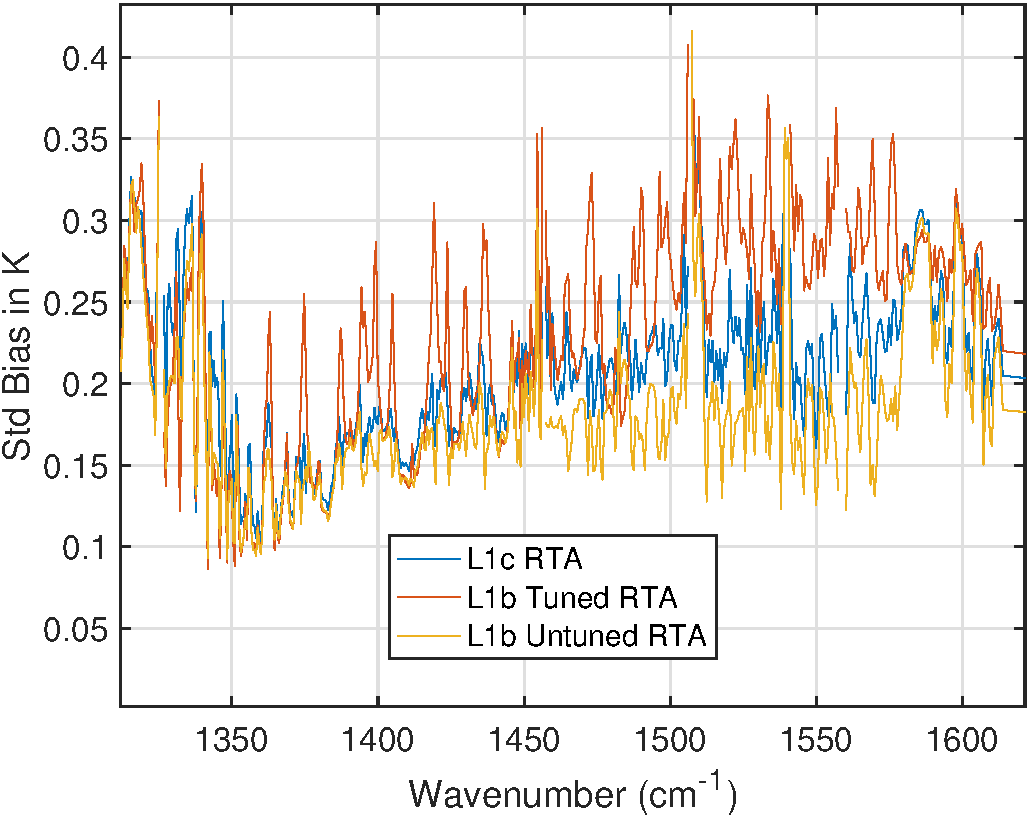
\includegraphics[width=0.65\linewidth]{./std_3rta_mw.pdf}
\end{center}
\end{frame}
\begin{frame}[label={sec:org6edc0cf}]{Midwave Bias Stds w/o L1btuning RTA}
Direct comparison L1c RTA versus L1b untuned RTA: HITRAN worse?
\begin{center}
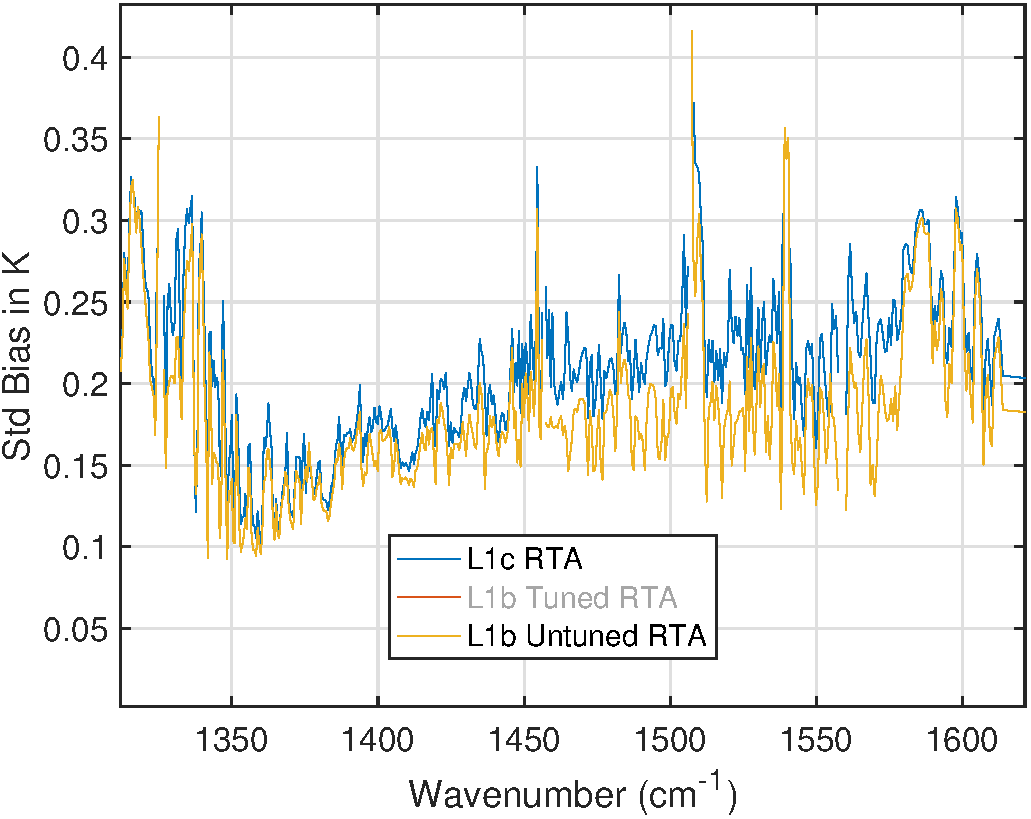
\includegraphics[width=0.75\linewidth]{./std_3rta_mw_noL1btuning.pdf}
\end{center}
\end{frame}
\begin{frame}[label={sec:org916b712}]{Midwave Bias Stds w/o L1b(untuned) RTA}
Direct comparison L1c RTA to L1b Tuned RTA: Tuning not catching scene variability?
\begin{center}
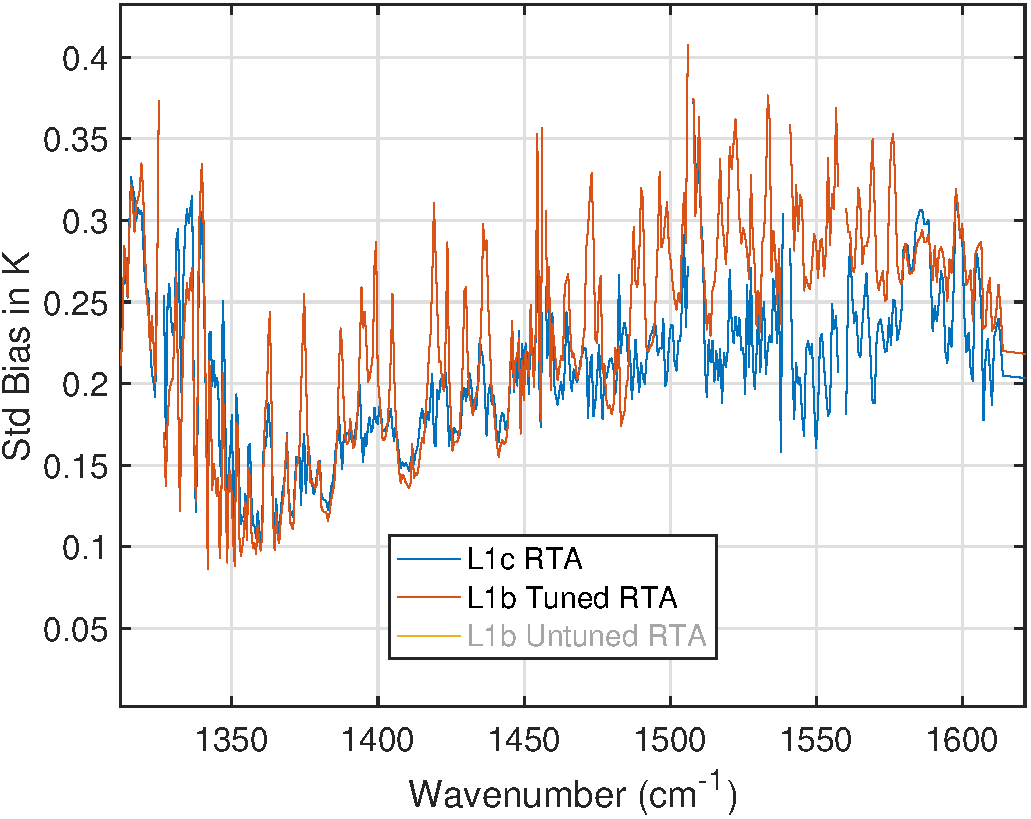
\includegraphics[width=0.75\linewidth]{./std_3rta_mw_nol1b untuned.pdf}
\end{center}
\end{frame}
\begin{frame}[label={sec:org8aa77db}]{1320-1614 \wn Bias Stds versus BTobs}
Scene dependence of STD, clear increase for cold scenes for L1b Tuned RTA
\begin{center}
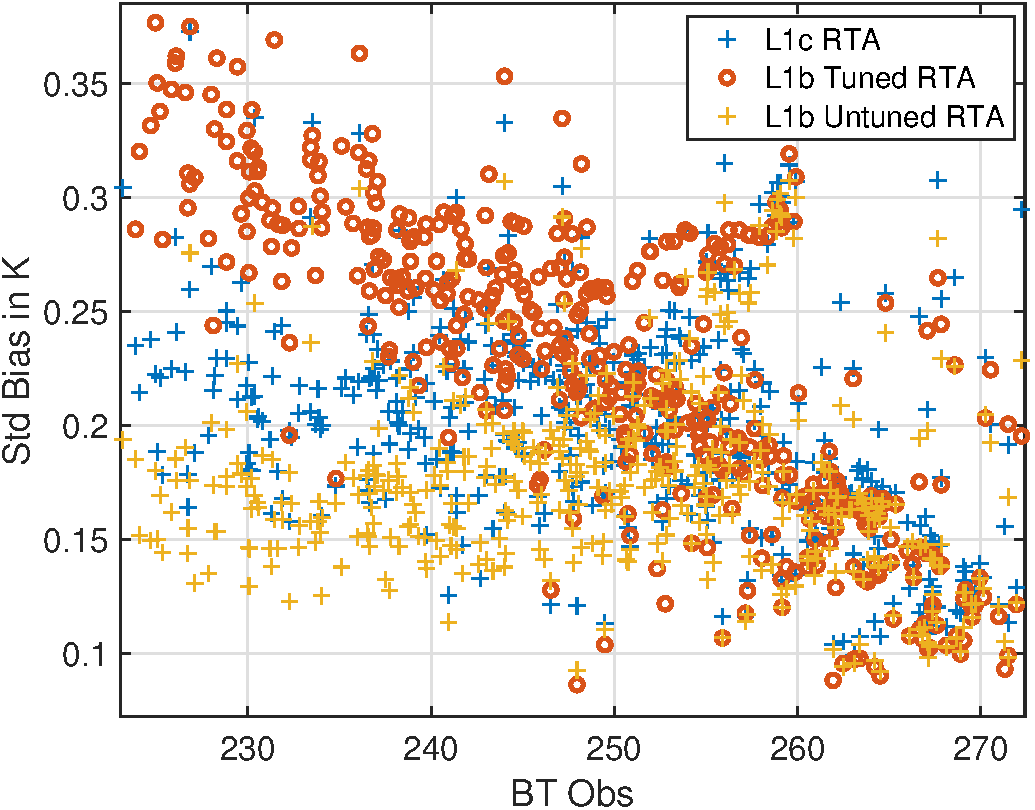
\includegraphics[width=0.75\linewidth]{./std_vs_btobs_1320-1614.pdf}
\end{center}
\end{frame}
\begin{frame}[label={sec:orgcfca8da}]{Final Effect: L1btuning RTA + Level 2 BT Tuning}
\begin{itemize}
\item V6 Level 2 retrieval uses tuned RTA \alert{BUT}
\item It also does BT tuning.
\item Except in longwave, they cancel each other out!  NOT GOOD.
\end{itemize}
\begin{center}
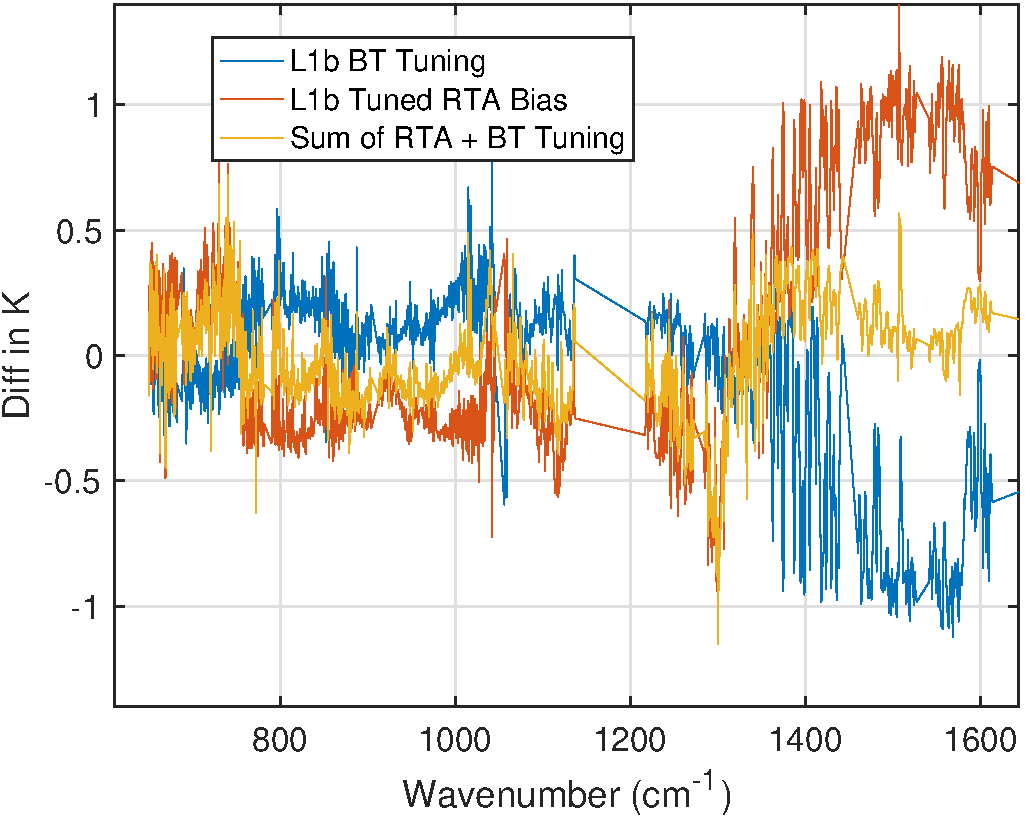
\includegraphics[width=0.65\linewidth]{./l1b_bttuning_l1b_tunedbias_added.pdf}
\end{center}
\end{frame}
\end{document}